This chapter investigates the effect of network structure on observed cooperation for the linear PGG described in \ref{ToTC}. The first section uses a simple lottery game to demonstrate the implementation of replicator dynamics. To this end, the paper \cite{RN30} is replicated and extended. \\

Then replicator dynamics are applied to the linear PGG. Under this regime, it is found that graphs with a power--law degree size distribution exhibit higher cooperation, when controlling for mean degree $m$. It is hypothesised that nodes with low degree size cooperate more, and the family of power--law models are characterised by a large number of low--degree nodes, resulting in higher overall cooperation than the WS and RRG model. \\
\section{Proof of Concept: Replicator and Imitation Dynamics} \label{Lottery_Me}
\subsection{Outline}
The paper chosen to replicate imitation and replicator dynamics was \cite{RN30}, which models a two-stage lottery game. Refer to \ref{Lottery} for a description of the game and the strategy space $S$. \\

The paper implemented agent--based replicator $(\alpha = 1)$ and imitation $(\alpha = 0)$ dynamics. After each round, every agent $i$ randomly chooses another agent $j$ from the population, and calculates $q_i$, \\

\begin{align} \label{rep}
q_i = \Bigg[ \frac{|\pi_j - \pi_i|}{\Delta} \Bigg]^\alpha \mathbbm{1}_{\{\pi_j>\pi_i\}}, \quad  0 \leq \alpha \leq 1.\end{align} 

In the formulation, $\Delta$ scales the difference so that $0 \leq q_i \leq 1$, and $\Delta = 16$ in this two-stage lottery game. Each agent then changes from strategy $i$ to strategy $j$ if $q_i \geq r_i,$ $r_i \sim \mathsf{U}(0,1)$. \\

\subsection{Results Comparison}
The simulated results were compared to the paper for $\alpha = 0, 1, 0.5$, and are shown below. \\

\FloatBarrier 
\begin{figure}[!h]
  \begin{subfigure}[b]{0.45\textwidth}
    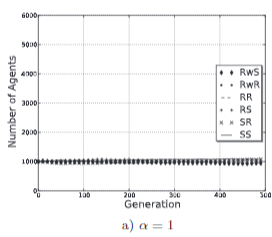
\includegraphics[width=\textwidth]{images/lottery1.png}
    \caption{Figure 5a from \cite{RN30}. The strategies SS, RR, SR, RS, R--WR, R--WS are represented by a solid line, crosses, plusses, dashes, dots and diamonds respectively. }
    \label{lottery1}
  \end{subfigure}
  \hfill
  \begin{subfigure}[b]{0.45\textwidth}
    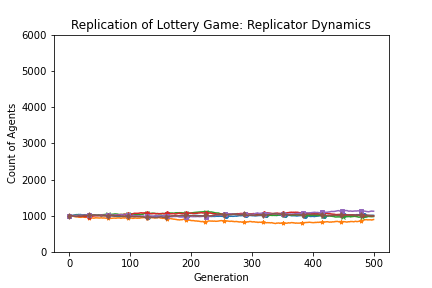
\includegraphics[width=1.25\textwidth]{images/lottery1_me.png}
    \caption{Replication of \ref{lottery1}. The strategies SS, RR, SR, RS, R--WR, R--WS are represented by blue circles, orange stars, green crosses, red pentagons, brown diamonds, and purple squares respectively.}
    \label{lottery1_me}
  \end{subfigure}
  \caption{Replication of Figure 5a from \cite{RN30}. The replication is successful, but these conditions do not provide anything interesting regarding replicator dynamics. Because the expected value of the strategies are equal, no strategy has an evolutionary advantage over any other.} \label{lottery_comp0}
\end{figure} 
\FloatBarrier

\FloatBarrier 
\begin{figure}[!h]
  \begin{subfigure}[b]{0.45\textwidth}
    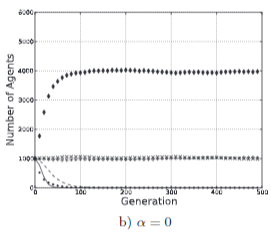
\includegraphics[width=\textwidth]{images/lottery2.png}
    \caption{Figure 5b from \cite{RN30}. The strategies SS, RR, SR, RS, R--WR, R--WS are represented by a solid line, crosses, plusses, dashes, dots and diamonds respectively. }
    \label{lottery2}
  \end{subfigure}
  \hfill
  \begin{subfigure}[b]{0.45\textwidth}
    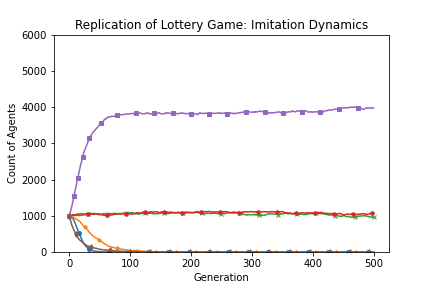
\includegraphics[width=1.25\textwidth]{images/lottery2_me.png}
    \caption{Replication of \ref{lottery2}. The strategies SS, RR, SR, RS, R--WR, R--WS are represented by blue circles, orange stars, green crosses, red pentagons, brown diamonds, and purple squares respectively.}
    \label{lottery2_me}
  \end{subfigure}
  \caption{Replication of Figure 5b from \cite{RN30}. The results are well replicated, and this model for imitation dynamics can be explored on other games.} \label{lottery_comp1}
\end{figure} 
\FloatBarrier



\FloatBarrier 
\begin{figure}[!h]
  \begin{subfigure}[b]{0.45\textwidth}
    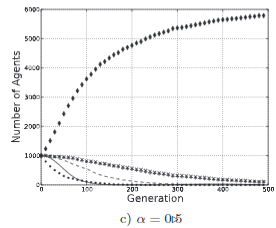
\includegraphics[width=\textwidth]{images/lottery3.png}
    \caption{Figure 5c from \cite{RN30}. The strategies SS, RR, SR, RS, R--WR, R--WS are represented by a solid line, crosses, plusses, dashes, dots and diamonds respectively. }
    \label{lottery3}
  \end{subfigure}
  \hfill
  \begin{subfigure}[b]{0.45\textwidth}
    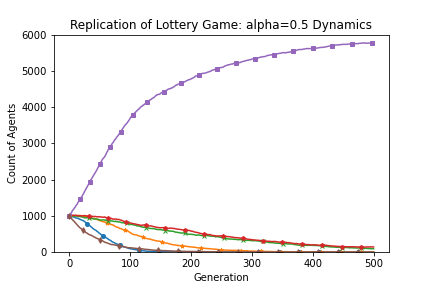
\includegraphics[width=1.25\textwidth]{images/lottery3_me.png}
    \caption{Replication of \ref{lottery3}. The strategies SS, RR, SR, RS, R--WR, R--WS are represented by blue circles, orange stars, green crosses, red pentagons, brown diamonds, and purple squares respectively. }
    \label{lottery3_me}
  \end{subfigure}
  \caption{Replication of Figure 5c from \cite{RN30}. This is neither true imitation or replicator dynamic, but provides an intermediary case.} \label{lottery_comp2}
\end{figure} 
\FloatBarrier


 It is also interesting to examine the results when the lottery win probability $p$ is not 0.5. For replicator dynamics, the strategy with the highest expected value eventually wins out, but for imitation dynamics the result is not so obvious. This was shown in Figure 6 from \cite{RN30}, and replicated below. For $p=0.4$, the expectation--maximising strategy is SS, but R--WS has an evolutionary advantage and takes over the population. This is supported by theoretical results in \cite{RN30}. Similarly, for $p=0.55$, the expectation--maximising strategy is RR, but R--WS also takes over the population. \\
 
 \FloatBarrier 
\begin{figure}[!h]
  \begin{subfigure}[b]{0.45\textwidth}
    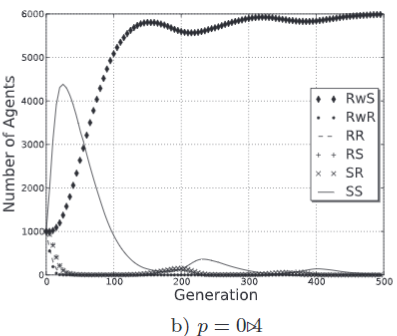
\includegraphics[width=\textwidth]{images/lotteryp4.png}
    \caption{Figure 6b from \cite{RN30}. The strategies SS, RR, SR, RS, R--WR, R--WS are represented by a solid line, crosses, plusses, dashes, dots and diamonds respectively.}
    \label{lotteryp4}
  \end{subfigure}
  \hfill
  \begin{subfigure}[b]{0.45\textwidth}
    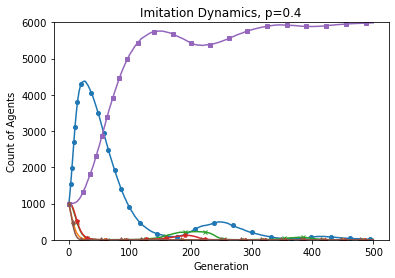
\includegraphics[width=1.25\textwidth]{images/lotteryp4_me.png}
    \caption{Replication of \ref{lotteryp4}. The strategies SS, RR, SR, RS, R--WR, R--WS are represented by blue circles, orange stars, green crosses, red pentagons, brown diamonds, and purple squares respectively. }
    \label{lotteryp4_me}
  \end{subfigure}
  \caption{Replication of Figure 6b from \cite{RN30}. Although SS is the expectation--maximising strategy, it is not an ESS, and R--WS has the evolutionary advantage.} \label{lottery_comp4}
\end{figure} 
\FloatBarrier

 \FloatBarrier 
\begin{figure}[!h]
  \begin{subfigure}[b]{0.45\textwidth}
    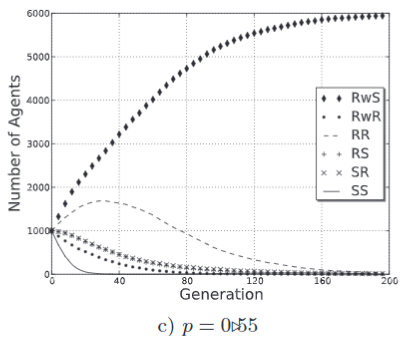
\includegraphics[width=\textwidth]{images/lotteryp055.png}
    \caption{Figure 6c from \cite{RN30}. The strategies SS, RR, SR, RS, R--WR, R--WS are represented by a solid line, crosses, plusses, dashes, dots and diamonds respectively.}
    \label{lotteryp055}
  \end{subfigure}
  \hfill
  \begin{subfigure}[b]{0.45\textwidth}
    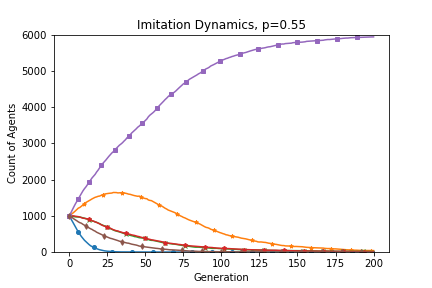
\includegraphics[width=1.25\textwidth]{images/lotteryp055_me.png}
    \caption{Replication of \ref{lotteryp055}. The strategies SS, RR, SR, RS, R--WR, R--WS are represented by blue circles, orange stars, green crosses, red pentagons, brown diamonds, and purple squares respectively. }
    \label{lotteryp4_me_2}
  \end{subfigure}
  \caption{Replication of Figure 6c from \cite{RN30}. In this case, RR is expectation--maximising, but R--WS still takes over the population.} \label{lottery_comp5}
\end{figure} 
\FloatBarrier

\subsection{Extension}
In \cite{RN30}, plots for $p=0.3, 0.7$ were also shown, however the expectation--maximising strategies win out quickly, so they are not included here. It is notable that in Figure \ref{lotteryp4_me}, there are some fluctuations that occur before stability. This is investigated further. \\

Consider the three strategies RS, SS, R--WS under the $p=0.4$ regime. For simplicity, assume these three strategies complete the strategy space. Their distributions are shown below. \\
\begin{align*}
    \mathbb P_{\text{RS}}(x = \pi)  &= \begin{cases} 0.4 \quad \pi = 12 \\
    0.6 \quad \pi =4 
    \end{cases}, \\
        \mathbb P_{\text{R--WS}}(x = \pi)  &= \begin{cases} 0.4 \quad \pi = 12 \\
    0.24 \quad \pi =8 \\
    0.36 \quad \pi = 0\\
    \end{cases}, \\
    \mathbb P_{\text{SS}}(x = \pi)  &= \mathbbm{1}_{\pi = 8}.
\end{align*}
Under imitation dynamics, a strategy $i$ has an evolutionary advantage over $j$, $j \prec i$, if $\mathbb P(\pi_i > \pi_j) > \mathbb P(\pi_i < \pi_j)$. In the example above, RS $\prec$ SS $\prec$ R--WS $\prec$ RS, which is a cycle. In \ref{lotteryp4_me}, the strategy SS eliminates RS much faster than RS can eliminate R--WS, so SS temporarily grows, and then succumbs to R--WS. \\

This relationship can be expressed as as a set of difference equations. Call $\rho_{\text{RS},t}, \rho_{\text{R--WS},t}, \rho_{\text{SS},t}$ the proportion of each strategy present at time $t$. The boundary condition is $\rho_{\text{RS},t}+ \rho_{\text{R--WS},t}+ \rho_{\text{SS},t} = 1$, $\forall t \in [0,T]$. Denote $\mathcal F_t$ the natural filtration of $\rho_{\text{RS},t}, \rho_{\text{R--WS},t}, \rho_{\text{SS},t}$ at time $t$.  \\
\begin{align*}
    \mathbb E \big [\rho_{\text{RS},t+1}| \mathcal F_t \big ] &= \rho_{\text{RS},t} \Bigg [ \rho_{\text{R--WS},t} [\mathbb P (\pi_\text{RS} > \pi_{\text{R--WS}}) -\mathbb P (\pi_\text{RS} < \pi_{\text{R--WS}}) ] \\
    &+ \rho_{\text{SS},t} [\mathbb P (\pi_\text{RS} > \pi_{\text{SS}}) -\mathbb P (\pi_\text{RS} < \pi_{\text{SS}}) ] \Bigg ] \\
    &= \rho_{\text{RS},t}\Bigg [ \rho_{\text{R--WS},t}(0.456 - 0.396) + \rho_{\text{SS},t}(0.4 - 0.6)  \Bigg ] \\
    &= \rho_{\text{RS},t}\Bigg [ \rho_{\text{R--WS},t}(0.06) + \rho_{\text{SS},t}(-0.2)  \Bigg ]
\end{align*}
The same logic can be applied for the difference equations for$\rho_{\text{SS},t}, \rho_{\text{R--WS},t}$. \\
\begin{align*}
    \mathbb E \rho_{\text{R--WS},t+1} &= \rho_{\text{R--WS},t} \Bigg [ \rho_{\text{RS},t} [\mathbb P (\pi_\text{R--WS} > \pi_{\text{RS}}) -\mathbb P (\pi_\text{R--WS} < \pi_{\text{RS}}) ] \\
    &+  \rho_{\text{SS},t} [\mathbb P (\pi_\text{R--WS} > \pi_{\text{SS}}) -\mathbb P (\pi_\text{R--WSS} < \pi_{\text{SS}}) ] \Bigg ] \\
    &= \rho_{\text{R--WS},t}\Bigg [ \rho_{\text{RS},t}(0.396-0.456) + \rho_{\text{SS},t}(0.4 - 0.36)  \Bigg ] \\
    &= \rho_{\text{R--WS},t}\Bigg [ \rho_{\text{RS},t}(-0.06) + \rho_{\text{SS},t}(0.04)  \Bigg ] \\
    \mathbb E \rho_{\text{SS},t+1}&= \rho_{\text{SS},t}\Bigg [ \rho_{\text{RS},t}(0.2) + \rho_{\text{R--WS},t}(-0.04)  \Bigg ]
\end{align*}
This set of difference equations cannot be solved analytically, and the numerical simulation is the same as Figure \ref{lotteryp4_me}. Under imitation dynamics, once a strategy is eliminated it can never return, and the elimination of RS ensures the eventual dominance of R--WS. RS is eliminated because it has the highest pairwise death rate, as SS dominates it with a rate of 0.2. This is much larger than any other pairwise comparison rate.  \\

The difference equations have ignored the effect of the other strategies, as they are negligible, but they were included for simulation. The image in \ref{lotteryp4_me} is aggregated over 20 trials, and the time to elimination is quite variable. The empirical quantiles are shown below, instead computed over 120 trials.  \\

\FloatBarrier
\graphCap{lotteryp4_me_quantiles_empirical.png}{0.75}{Empirical 2.5\%, 97.5\% Quantiles of Imitation Dynamics Lottery Game, $p=0.4$, T = 120. The strategies SS, RR, SR, RS, R--WR, R--WS are represented by blue circles, orange stars, green crosses, red pentagons, brown diamonds, and purple squares respectively. The quantile for each series is the dashed line. }{lottery_quantiles_empirical}
\FloatBarrier
Figure \ref{lottery_quantiles_empirical} shows how great the variance of certain series are, particularly SS and R--WS. When R--WS is prominent and the strategies SR, RS are not extinct, SR, RS are able to grow. This occurs around the 200th generation. The strategy SS, which outperforms SR and RS, then dominates them. SS is dominated by R--WS, and this cycle continues until SR and RS are eliminated. The reason that they are eliminated is because the highest rate of dominance is SS over SR, RS. \\
\FloatBarrier
\graphCap{lotteryp4_me_quantiles.png}{0.75}{95\% Confidence Interval for the Mean, Imitation Dynamics Lottery Game, $p=0.4$, T = 120. The strategies SS, RR, SR, RS, R--WR, R--WS are represented by blue circles, orange stars, green crosses, red pentagons, brown diamonds, and purple squares respectively. The confidence interval for each series is the dashed line. }{lottery_quantiles}
\FloatBarrier
 The computed confidence intervals assume a normal distribution of the mean under the Central Limit Theorem. The computed standard deviation of each point in the time series is used as an estimate of the true standard deviation. Because the number of trials $T=120$, the confidence interval is tight around the sample mean. The original paper uses $T=20$, which results in a confidence interval four times as wide Figure \ref{lottery_quantiles}. Therefore it is suggested that more than 20 trials are used for future samples. \\



\subsection{Summary}
The purpose of replicating \cite{RN30} was to demonstrate replicator and imitation dynamics. This demonstration was achieved, and now these dynamics can be applied to the PGG. A cycle of strategies was demonstrated for imitation dynamics under a $p=0.4$ regime. Although the original paper did not investigate the distribution of results, they are discussed above. The paper \cite{RN30} did not use an underlying network structure, but the dynamics can easily be transposed onto a graph by limiting the sample space of agents to neighbours. \\


\section{Local Replicator Dynamics for Public Good Games}
\subsection{Outline}
The following section investigates the effect of graph model on cooperation under local replicator dynamics. The graph models from \ref{other_networks} are also investigated here, and sample characteristics are given in Table \ref{graph_stats}. The game is played by a population of 500 agents, where each agents hosts a play of the PGG with their neighbours. After every agent has hosted, the agent--based replicator dynamics from equation \eqref{rep} are implemented for each agent. Each plot aggregates the mean of each series over 80 trials. \\

It is found that the graphs with a power--law degree size distribution induce higher cooperation. The effect of $C_\Delta$ is isolated under a power--law degree size distribution by using a new model type, PL, and is also examined in the WS family of graph models. Under the PL model, higher $C_\Delta$ weakly induces higher cooperation, while the trend is reversed for the WS family of models. \\

Then the effect of targeted mean degree $m$ is examined for RRG and BA models. Both of these experiments indicate that higher $m$ lead to lower cooperation. Finally, the cooperation levels are stratified by degree size within a BA graph model. This experiments shows that the nodes with low degree size have a higher contribution proportion than average, which may explain the trend. \\

\subsection{Results}
\FloatBarrier
\graphCap{replicator_graphs_low}{0.8}{Comparing Graph Models: Replicator Dynamics. Trend for $r \in \{2, 2.5, 3, 3.5\}$. In each graph, the blue circles, orange stars, green crosses, and red pentagons correspond to the WS model, TAG model, BA model, and RRG model respectively. }{replicator_low} 
\FloatBarrier
\graphCap{replicator_graphs_medium}{0.8}{Comparing Graph Models: Replicator Dynamics. Trend for $r \in \{4,4.5,5,5.5\}$. In each graph, the blue circles, orange stars, green crosses, and red pentagons correspond to the WS model, TAG model, BA model, and RRG model respectively. }{replicator_medium}
\FloatBarrier
\graphCap{replicator_graphs_large}{0.8}{Comparing Graph Models: Replicator Dynamics. Trend for $r \in \{6,6.5,7,7.5\}$. In each graph, the blue circles, orange stars, green crosses, and red pentagons correspond to the WS model, TAG model, BA model, and RRG model respectively. }{replicator_large}\FloatBarrier

Replicator dynamics result in slower convergence than the satisfaction model in Chapter \ref{TA}. Therefore the number of generations has been extended to 200, so that equilibrium is observed. Figure \ref{replicator_low} shows the TAG and BA model inducing higher cooperation than WS, RRG models. This trend continues for $2.5 \leq r \leq 7.5$. It appears that graph models with a power law degree size distribution induce higher cooperation. The results discussed in Chapter \ref{C1} corroborate this trend. \\

There is insufficient information to determine if the clustering coefficient $C_\Delta$ influences cooperation, because the graph models are too varied. Therefore, it will need to be tested in isolation.\\

\subsection{Isolating the Effect of Clustering Coefficient: Power Law Degree Size Distribution}
To test the hypothesis that the average clustering coefficient $C_\Delta$ does not impact cooperation, the \verb+power_law+ model was used to create another graph model, denoted PL. It induces a degree distribution with power law shape, but the parameter $p$ dictates the clustering coefficient. After each node is connected, the parameter $p$ determines the probability that the next link joins two neighbours, completing the triangle. Two degree histograms are plotted below, which emphasise the degree size distribution. \\
\FloatBarrier
\graphCap{PL01BA.png}{0.5}{Comparison of Power Law Clustering Graph with BA model, $p=0.1$. The degree histograms are similar, so the only difference is the clustering coefficient.}{PL01BA}
\FloatBarrier
\graphCap{PL05BA.png}{0.5}{Comparison of Power Law Clustering Graph with BA model, $p=0.5$. The degree histograms are similar, so the only difference is the clustering  coefficient.}{PL05BA}
\FloatBarrier
The summary statistics are also reported. It is important to note the only statistic that noticeably changes is $C_\Delta$, as desired. \\
\FloatBarrier
\begin{table}[!h]
\begin{center}
\begin{tabular}{|l|l|l|l|l|}
\hline
Graph Type & Mean Degree & $l$ & $C_\Delta$ & Degree Variance \\ \hline
PL: $p=0.1$        & 5.96        & 3.234                         & 0.10                   & 42.35           \\ \hline
PL: $p=0.2$        & 5.96           & 3.24                         & 0.15                   & 44.07               \\ \hline
PL: $p=0.3$       & 5.96        & 3.23                       & 0.20                   & 46.28           \\ \hline
PL: $p=0.4$       & 5.96        & 3.25                         & 0.25                   & 47.92           \\ \hline
PL: $p=0.5$         & 5.96           & 3.26                         & 0.30                   & 50.47            \\ \hline
\end{tabular}
\caption{Computed characteristics for PL graph, varying cluster parameter $p$. The characteristics were computed over 100 samples of each graph, and then averaged. } \label{graph_stats}
\end{center}
\end{table}
\FloatBarrier
\graphCap{comparing_power_p_low.png}{0.8}{To test the effect of $C_\Delta$, the parameter $p$ in a PL graph was varied. In each graph, the blue circles, orange stars, green crosses, red pentagons, and purple squares correspond to $p=[0.1,0.2,0.3,0.4,0.5]$ respectively. The observed trend is that higher $C_\Delta$ leads to marginally higher cooperation.}{power_p_low}
\FloatBarrier
\graphCap{comparing_power_p_high.png}{0.8}{To test the effect of $C_\Delta$, the parameter $p$ in a PL graph was varied. In each graph, the blue circles, orange stars, green crosses, red pentagons, and purple squares correspond to $p=[0.1,0.2,0.3,0.4,0.5]$ respectively. The trend is unclear here, because $r=2.75, 3.5$ indicate higher $C_\Delta$ leads to higher cooperation, but that trend is not observed in for $r=3.0,3.25$.}{power_p_high} \FloatBarrier

These tests indicate that, when controlling for degree size distribution, the clustering coefficient $C_\Delta$ may have a marginal effect. The correlation is weakly positive, and is much more evident for $1.75\leq r\leq 3.0$. It is also necessary to test the effect of $C_\Delta$ under a different degree size distribution. \\

\subsection{Isolating the Effect of Clustering Coefficient: Constant Degree Size Distribution}
The WS model is a family of graphs, characterised by rewiring probability $p$. By increasing $p$, the $l$ statistic is reduced while $C_\Delta$ remains high for $0\leq p\leq0.15$. However there exists a region for $p$ where $C_\Delta$ decreases and $l$ does not change as rapidly. It is this region that will be isolated to test the effect of local clustering on cooperation in graphs under a near--constant degree distribution regime. Recall that a WS graph starts with a circle of nodes, each node connected to its adjacent $\frac{m}{2}$ circular neighbours. Hence the initial degree is $m$ for each node, and this only varies marginally due to $p$. There are certainly no scale factors such as in the PL, BA, or TAG models. \\

\FloatBarrier
\begin{table}[!h]
\begin{center}
\begin{tabular}{|l|l|l|l|l|}
\hline
Graph Type & Mean Degree & $l$ & $C_\Delta$ & Degree Variance \\ \hline
WS: $p=0.1$        & 6        & 5.41                         & 0.44                  & 0.57           \\ \hline
WS: $p=0.2$        &6           & 4.53                         & 0.316                   & 1.06               \\ \hline
WS: $p=0.3$        &6           & 4.16                         & 0.22                   & 1.51               \\ \hline
WS: $p=0.4$       & 6        & 3.95                         & 0.14                  & 1.93           \\ \hline
WS: $p=0.5$         & 6           & 3.83                         & 0.09                   & 2.25            \\ \hline
\end{tabular}
\caption{Computed characteristics for WS graph, varying rewiring probability parameter $p$. The characteristics were computed over 100 samples of each graph, and then averaged. } \label{graph_stats_WS}
\end{center}
\end{table}
\FloatBarrier

\graphCap{graph_p_med.png}{0.8}{Effect of rewiring $p$ in a WS model. In each graph, the blue circles, orange stars, green crosses, red pentagons, and purple squares correspond to $p=[0.1,0.2,0.3,0.4,0.5]$ respectively. The trend indicates that higher $p$ leads to higher cooperation.}{graph_p_med}
\FloatBarrier
\graphCap{graph_p_high.png}{0.8}{Capt. In each graph, the blue circles, orange stars, green crosses, red pentagons, and purple squares correspond to $p=[0.1,0.2,0.3,0.4,0.5]$ respectively. The same trend is observed here.}{graph_p_high}
\FloatBarrier
Figures \ref{graph_p_med} and \ref{graph_p_high} indicate that higher rewiring probability $p$ leads to higher cooperation. This indicates that lowering the clustering coefficient induces higher cooperation, a contradiction to Figures \ref{power_p_low} and \ref{power_p_high}. In those figures, there was a weak positive correlation between $C_\Delta$ and cooperation. At this stage, there is no feasible explanation for this discrepancy, so further investigation is required. \\

\subsection{The Effect of Mean Degree: RRG}
The initial experiments indicated that graphs with a power law degree distribution induced higher cooperation. This may be because they include nodes with higher degree. It is of interest to isolate the effect of higher degree on cooperation. To do this, a family of RRG are sampled, and the mean degree is varied between 4 and 8. \\


\graphCap{RRG_graph_m_med.png}{0.8}{The effect of mean degree, RRG model. In each graph, the blue circles, orange stars, green crosses, red pentagons, and purple squares correspond to $m =  [4,6,8,10,12]$ respectively. }{graph_m_low} \FloatBarrier

\graphCap{RRG_graph_m_high.png}{0.8}{The effect of mean degree, RRG model. In each graph, the blue circles, orange stars, green crosses, red pentagons, and purple squares correspond to $m =  [4,6,8,10,12]$ respectively. }{graph_m_med} \FloatBarrier

The plots above dissect the effect of increasing average degree across the whole graph. The trend is that higher degree leads to less cooperation. This trend is consistent across $3.0\leq r\leq6.5$. This indicates that the trend observed in Figure \ref{replicator_low} is not due to the power--law graphs having some nodes with higher degree, but must be explained in a different manner. These results can also be tested on a BA model. \\
\FloatBarrier
\graphCap{BA_graph_m_low.png}{0.8}{The effect of mean degree, BA model. In each graph, the blue circles, orange stars, green crosses, red pentagons, and purple squares correspond to $m = [4,6,8,10,12]$ respectively.}{BA_graph_m_low}
\FloatBarrier
\graphCap{BA_graph_m_med.png}{0.8}{The effect of mean degree, BA model. In each graph, the blue circles, orange stars, green crosses, red pentagons, and purple squares correspond to $m = [4,6,8,10,12]$ respectively.}{BA_graph_m_med}
\FloatBarrier
Across Figures \ref{graph_m_low}, \ref{graph_m_med},\ref{BA_graph_m_low}, and \ref{BA_graph_m_med} there is a consistent trend that higher targeted mean degree $m$ leads to lower cooperation. A plausible explanation is the \emph{scaled effect} of $r$. For an agent $i$ hosting a game of size $|N_i|$ with each agent defecting, then $\lceil \frac{|N_i|}{r}\rceil$ can be viewed as the number of agents who must start cooperating to ensure cooperation is the most profitable strategy. This is increasing in $|N_i|$, which lends credence to the hypothesis that lower degrees have a higher proportion of cooperators. It is also feasible that a node with low degree can be surrounded by cooperators, and become \emph{immune} to defection much faster than a high--degree node. This trend is very consistent across both models and varying $r$. \\

It also suggests that the increase in cooperation of the power--law graphs observed in Figures \ref{replicator_low}, \ref{replicator_medium}, and \ref{replicator_large} is not due to the high--degree nodes, but instead occurs because there exist a large proportion of nodes with degree lower than the common $m$.  \\

The last effect to consider is stratifying the nodes by degree within a single graph model. To do this, the BA model was used, and the cooperation level recorded for each nodes, then aggregated by degree. \\

\subsection{Cooperation Level Within a Single Graph Instance: BA model }
This experiment seeks to stratify the cooperation level of each point according to its degree. Earlier experiments indicated that increasing the targeted mean degree $m$ reduces cooperation, but that was measuring the whole--model cooperation. Instead, $m, r$ are fixed, and the cooperation level at the final step for each node is examined, and then aggregated over all nodes with that degree. \\
\FloatBarrier
\graphCap{BA_degree_groups_30.png}{0.8}{Cooperation vs Node Degree: BA Model, $r=3.0$. The bar chart, plotted on the left axis, is a histogram of the degree size. On the right axis, and plotted in black, is the final cooperation level of all nodes according to their degree. The mean cooperation is plotted as red horizontal line, for comparison. }{BA_groups_low}
\FloatBarrier

\FloatBarrier
\graphCap{BA_degree_groups_45.png}{0.8}{Cooperation vs Node Degree: BA Model, $r=4.5$. The bar chart, plotted on the left axis, is a histogram of the degree size. On the right axis, and plotted in black, is the final cooperation level of all nodes according to their degree. The mean cooperation is plotted as red horizontal line, for comparison. }{BA_groups_med}
\FloatBarrier

These figures demonstrate that the lower degree nodes contribute a greater fraction than the mean. The higher nodes are incentivised to defect, as their gain from defection can be very high. It is notable that this strategy does not propagate well, and even for low $r$ high cooperation is achieved. These results corroborate the findings in Figures \ref{BA_graph_m_low} and \ref{BA_graph_m_med}, which show that there is higher cooperation amongst lower degrees. \\

\subsection{Summary}
Four graph models were examined under replicator dynamics, and the results are plotted in Figures \ref{replicator_low}, \ref{replicator_medium}, and \ref{replicator_large}. The trend of these plots was that the models with power--law degree size distribution, specifically the BA and TAG models, induced higher cooperation. In an attempt to explain these results, several more experiments were carried out. \\

Firstly, the effect of $C_\Delta$ was examined for both a power--law graph (PL), and also the WS family of models. These produced weakly contradictory results. Under the WS model, increasing $C_\Delta$ reduced cooperation. Under the PL model, it was more unclear but it appears that increasing $C_\Delta$ weakly increases cooperation. At this stage, there is no explanation for these effects. \\

Then the effect of targeted mean degree $m$ was examined. This produced strong results across both the BA and RRG models, demonstrating that mean degree is negatively correlated to cooperation level. This gives some suggestion for the trends observed in Figures \ref{replicator_low}, \ref{replicator_medium}, and \ref{replicator_large}. Because the BA and TAG model have a power--law degree size distribution with the same mean degree $m$ as the WS, RRG models, they necessarily have a lot of nodes with degree less than $m$. These nodes cooperate more often than their higher degree size counterparts, so induce higher mean cooperation. 
